%% DONE
\id{МРНТИ 28.17.19}{https://doi.org/10.58805/kazutb.v.1.26-878}

\begin{articleheader}
\sectionwithauthors{А.Т. Мазакова, Ш.А. Джомартова, Б.М. Мазакова, М.С. Алиаскар, Е.К. Мергенгали, Т.Ж. Мазаков, А.Т. Досаналиева, А.Д. Майлыбаева}{ПРОГНОЗИРОВАНИЕ ПОСЛЕДСТВИЙ СЕЛЕВОГО ПРОРЫВА С УЧЕТОМ ХАРАКТЕРИСТИК ВОДОЕМА}

{\bfseries
\textsuperscript{1}А.Т. Мазакова\authorid,
\textsuperscript{1}Ш.А. Джомартова\authorid,
\textsuperscript{2}Б.М. Мазакова\authorid,
\textsuperscript{3}М.С. Алиаскар\authorid,
\textsuperscript{1}Е.К. Мергенгали\authorid,
\textsuperscript{1,3}Т.Ж. Мазаков\textsuperscript{\envelope } \authorid,
\textsuperscript{4}А.Т. Досаналиева\authorid,
\textsuperscript{5}А.Д. Майлыбаева\authorid}
\end{articleheader}

\begin{affiliation}
\emph{¹Казахский национальный университет имени аль-Фараби, Алматы, Казахстан,}

\emph{\textsuperscript{2}Казахский агротехнический исследовательский университет имени С. Сейфуллина, Астана, Казахстан,}

\emph{\textsuperscript{3}Международный инженерно-технологический университет, Алматы, Казахстан,}

\emph{\textsuperscript{4}Алматинский Технологический Университет, Алматы, Казахстан,}

\emph{\textsuperscript{5}Атырауский универститет имени Х. Досмухамедова}

\raggedright \textsuperscript{\envelope }\emph{Корреспондент-автор: tmazakov@mail.ru}
\end{affiliation}

Весной 2010 года в Алматинской области, в 2014 году в Карагандинской
области, а также в начале 2024 года в северных регионах Казахстана
произошли разрушительные наводнения, сопровождавшиеся человеческими
жертвами и значительным ущербом. Эти события подчеркнули необходимость
создания эффективных систем мониторинга для гидротехнических сооружений.

Современные системы мониторинга гидрологической ситуации на водоемах
позволяют заранее выявлять потенциальные угрозы для человека и
окружающей среды. Основная цель мониторинга заключается в предоставлении
точных данных, необходимых для прогнозирования чрезвычайных ситуаций.
Проектирование таких систем включает разработку и анализ математических
моделей, способных в режиме реального времени рассчитывать объем воды,
который может вместить водоем, а также предсказывать момент его
заполнения и угрозы прорыва плотины. Применение таких систем
способствует принятию оперативных мер по обеспечению экологической
безопасности.

В данной работе представлена система прогнозирования, способная
оценивать последствия селевых прорывов. Разработанная система базируется
на методах математического моделирования. В отличие от аналогов,
предложенная модель учитывает, как параметры водоема, так и особенности
русла реки.

Для внедрения системы в практику создано программное обеспечение на
языке Python. Проведенные эксперименты показали, что модель достоверно
отражает реальные условия и может успешно применяться в различных
сценариях.

{\bfseries Ключевые слова:} бьеф, математическая модель, плотина,
прогнозирование, сель.

\begin{articleheader}
{\bfseries СУ ОБЪЕКТІНІҢ СИПАТТАРЫН ЕСКЕ АЛУ МЕН СЕЛДІҢ САЛДАРЫН БОЛЖАУ}

{\bfseries
\textsuperscript{1}Ә.Т. Мазақова,
\textsuperscript{1}Ш.А. Джомартова,
\textsuperscript{2}Б.М. Мазакова,
\textsuperscript{3}М.С. Әлиасқар,
\textsuperscript{1}Е.К. Мергенгали,
\textsuperscript{1,3}Т.Ж. Мазақов\textsuperscript{\envelope },
\textsuperscript{4}А.Т. Досаналиева,
\textsuperscript{5}А.Д.Майлыбаева}
\end{articleheader}

\begin{affiliation}
\emph{\textsuperscript{1}Әл-Фараби атындағы Қазақ ұлттық университеті, Алматы, Қазақстан,}

\emph{\textsuperscript{2}Сейфуллин атындағы Қазақ агротехникалық зерттеу университеті, Астана, Қазақстан,}

\emph{\textsuperscript{3}Халықаралық инженерлік және технология университеті, Алматы, Қазақстан,}

\emph{\textsuperscript{4}Алматы технологиялық университеті, Алматы, Қазақстан,}

\emph{\textsuperscript{5}Досмұхамедов атындағы Атырау университеті,}

\emph{e-mail:} \emph{tmazakov@mail.ru}
\end{affiliation}

2010 жылдың көктемінде Алматы облысында, 2014 жылы Қарағанды
\hspace{0pt}\hspace{0pt}облысында, ал 2024 жылдың басында Қазақстанның
солтүстік облыстарында адам шығынымен және айтарлықтай шығынмен қатар
жүретін жойқын су тасқыны болды. Бұл іс-шаралар гидротехникалық
құрылыстарды бақылаудың тиімді жүйелерінің қажеттілігін көрсетті.

Су объектілеріндегі гидрологиялық жағдайды бақылаудың заманауи жүйелері
адам мен қоршаған ортаға ықтимал қауіптерді алдын ала анықтауға
мүмкіндік береді. Мониторингтің негізгі мақсаты -- төтенше жағдайларды
болжауға қажетті нақты мәліметтерді қамтамасыз ету. Мұндай жүйелерді
жобалау нақты уақыт режимінде резервуар ұстай алатын су көлемін
есептеуге, сондай-ақ оны толтыру сәтін және бөгеттің бұзылу қаупін
болжауға қабілетті математикалық модельдерді әзірлеуді және талдауды
қамтиды. Мұндай жүйелерді пайдалану экологиялық қауіпсіздікті қамтамасыз
ету бойынша жедел шараларды қабылдауға ықпал етеді.

Бұл жұмыста селдің салдарын бағалауға қабілетті болжау жүйесі ұсынылған.
Әзірленген жүйе математикалық модельдеу әдістеріне негізделген. Өзінің
аналогтарынан айырмашылығы, ұсынылған модель су қоймасының параметрлерін
де, өзен арнасының ерекшеліктерін де ескереді.

Жүйені тәжірибеге енгізу үшін Python тілінде бағдарламалық жасақтама
жасалды. Жүргізілген эксперименттер модель нақты жағдайларды сенімді
түрде көрсететінін және әртүрлі сценарийлерде сәтті қолданыла алатынын
көрсетті.

{\bfseries Түйін сөздер:} бассейн, математикалық модель, бөгет, болжау,
сел.

\begin{articleheader}
{\bfseries FORECASTING THE CONSEQUENCES OF A MUDFLOW TAKING INTO ACCOUNT
THE CHARACTERISTICS OF THE WATER BODY}

{\bfseries \textsuperscript{1}A.T. Mazakova,
\textsuperscript{1}Sh.A. Jomartova,
\textsuperscript{2}B.M. Mazakova,
\textsuperscript{3}M.S. Aliaskar,
\textsuperscript{1}Y.К. Mergengali,
\textsuperscript{1,3}T.Zh. Mazakov\textsuperscript{\envelope },
\textsuperscript{4}A.T.Dossanalyieva,
\textsuperscript{5}A.D.Mailybayeva}
\end{articleheader}

\begin{affiliation}
\emph{¹Kazakh National University named after Al-Farabi, Almaty, Kazakhstan,}

\emph{\textsuperscript{2}Kazakh Agrotechnical Research University named after S. Seifullin, Astana, Kazakhstan,}

\emph{\textsuperscript{3}International Engineering and Technology University, Almaty, Kazakhstan,}

\emph{\textsuperscript{4}Almaty Technological University, Almaty, Kazakhstan,}

\emph{\textsuperscript{5}Atyrau University named after Kh. Dosmukhambetov,}

\emph{e-mail:} \emph{tmazakov@mail.ru}
\end{affiliation}

In the spring of 2010 in the Almaty region, in 2014 in the Karaganda
region, and in early 2024 in the northern regions of Kazakhstan,
devastating floods occurred, accompanied by human casualties and
significant damage. These events emphasized the need to create effective
monitoring systems for hydraulic structures.

Modern systems for monitoring the hydrological situation on water bodies
allow early detection of potential threats to humans and the
environment. The main goal of monitoring is to provide accurate data
necessary for forecasting emergency situations. Designing such systems
includes the development and analysis of mathematical models capable of
calculating in real time the volume of water that a water body can hold,
as well as predicting the moment of its filling and the threat of a dam
break. The use of such systems facilitates the adoption of prompt
measures to ensure environmental safety.

This paper presents a forecasting system capable of assessing the
consequences of mudflows. The developed system is based on mathematical
modeling methods. Unlike analogues, the proposed model takes into
account both the parameters of the reservoir and the features of the
river bed.

To implement the system in practice, software was created in Python. The
experiments showed that the model reliably reflects real conditions and
can be successfully applied in various scenarios.

{\bfseries Keywords:} pool, mathematical model, weir, forecasting, mudflow.

\begin{multicols}{2}
{\bfseries Актуальность.} За последнее столетие в мире произошло множество
катастроф, связанных с разрушением гидротехнических сооружений, которые
сопровождались человеческими жертвами и значительными экономическими
потерями.

Одной из наиболее трагических стала авария на плотине Сент-Франсис в
Калифорнии, произошедшая в марте 1928 года, когда погибло более 600
человек. В 1963 году обрушение горного массива в водохранилище Вайонт
(Италия) вызвало гигантские волны высотой до 70 метров, которые
разрушили четыре населенных пункта и привели к гибели 4400 человек.
Наводнение в Краснодарском крае в июле 2002 года, повлекшее разрушение
гидроузла, стало причиной гибели 114 тысяч человек и нанесло
экономический ущерб, оцененный в 15 миллиардов рублей {[}1-2{]}.

17 августа 2009 года на Саяно-Шушенской ГЭС произошла крупная авария,
унесшая жизни 75 человек. В результате были серьезно повреждены
оборудование и инфраструктура станции. Авария вызвала негативные
изменения в экологической ситуации прилегающей акватории, а также
оказала значительное влияние на социально-экономическое состояние
региона и страны в целом {[}3{]}.

Современные мониторинговые системы должны обеспечивать постоянное
наблюдение за природными и техногенными процессами, чтобы заранее
выявлять потенциальные угрозы для жизни человека и окружающей среды.
Основная задача мониторинга заключается в предоставлении точной
информации, необходимой для прогнозирования чрезвычайных ситуаций. Для
этого необходимо объединять интеллектуальные, информационные и
технологические ресурсы различных организаций и ведомств, отвечающих за
мониторинг специфических опасностей.

Проектирование мониторинговых систем требует разработки и анализа
математических моделей, способных в реальном времени определять объем
воды, который может вместить водоем, а также прогнозировать время до его
заполнения (до уровня гребня плотины). Эти данные являются критически
важными для своевременного предупреждения населения и органов власти,
что позволяет оперативно принимать меры по обеспечению экологической
безопасности.

Таким образом, исследования, направленные на разработку математических
моделей для оценки прорыва дамб и создание надежных средств защиты
информации, остаются весьма актуальными.

{\bfseries Введение.} В Казахстане насчитывается 1665 гидротехнических
сооружений, включая 319 водохранилищ объемом более 1,0 млн м³. Из них в
республиканской собственности находится 83 объекта, в коммунальной --
200, в частной -- 34, а 60 водохранилищ являются бесхозяйными. Среди 443
плотин 32 находятся в республиканской собственности, 346 -- в
коммунальной, 45 -- в частной, а 20 остаются бесхозяйными. Также
эксплуатируются 125 дамб и 778 других гидротехнических сооружений.

Среди крупных водохранилищ выделяются Астанинское (1970 г., объем 410,9
млн м³), Селетинское (1965 г., 230 млн м³), Каргалинское (1975 г., 280
млн м³), Бартогайское (1982 г., 320 млн м³), Капшагайское (1970 г., 18
560 млн м³), Терс-Ащибулакское (1963 г., 158,6 млн м³), Тасоткельское
(1974 г., 620 млн м³), Самаркандское (1939 г., 253,7 млн м³),
Верхне-Тобольское (1972 г., 816,6 млн м³), Каратомарское (1965 г., 586
млн м³), Бугуньское (1967 г., 370 млн м³) и другие.

Большинство водохранилищ и гидроузлов (около 60\%) находятся в
коммунальной собственности, в том числе на балансе Казводхоза, а около
20\% объектов принадлежат отделам сельского хозяйства акиматов. Эта
ситуация указывает на нерешенность вопроса об окончательной
принадлежности данных объектов. В течение последних 10--15 лет около
20\% водохранилищ были переданы в аренду частным лицам, преимущественно
для нужд сельского хозяйства, рыбоводства и рекреации. Однако только в
отдельных случаях аренда приносит положительные результаты, поскольку
частным арендаторам часто не хватает средств для ремонта ключевых
сооружений {[}4{]}.

\begin{figure}[H]
	\centering
	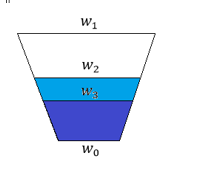
\includegraphics[width=0.6\columnwidth]{media/ict/image2}
	\caption*{Рис. 1 - Вид водоема со стороны плотины}
\end{figure}

Весной 2010 года в Алматинской области произошло разрушительное
наводнение, вызванное прорывом плотины, повлекшее человеческие жертвы и
масштабные разрушения. Подобное трагическое событие повторилось в 2014
году в Карагандинской области. Эти катастрофы стали серьезным
предупреждением для страны и подчеркнули важность предотвращения таких
ситуаций в будущем {[}5{]}.

{\bfseries Материалы и методы.} В математической модели рассмотрен
трапецеидальный тип водоема, вид которого со стороны плотины представлен
на рисунке 1.

Введем следующие обозначения {[}6-8{]}:

\(\mathrm{\Delta}T\)- временной шаг отсчета (в часах);

\(l\) - длина водоема (в метрах)

\(\omega_{0}\) , \(S_{0}\) - ширина и площадь водоема по основанию;

\(\omega_{1}\) , \(S_{1}\) - ширина и площадь водоема по уровню гребня
плотины;

\(\omega_{2}\) , \(S_{2}\) - ширина и площадь водоема по поверхности
воды;

\(\omega_{3}\) , \(S_{3}\) - ширина и площадь водоема по верхней точки
прорана в плотине;

\(V_{0}\) -- общий объем водоема;

\(V_{1}\) -- незаполненный объем водоема;

\(V_{2}\) -- объем водоема от поверхности воды до верхней точки прорана
в плотине;

\(V_{3}\) -- объем водоема от нижней до верхней точки прорана в плотине;

\(\mathrm{\Delta}V_{1}\) - объем воды поступившей в водоем за время
\(\mathrm{\Delta}T\);

\(\mathrm{\Delta}V_{2}\) - объем воды вытекший из водоема за время
\(\mathrm{\Delta}T\);

\(\mathrm{\Delta}V\) - разница между объемами вытекшей и поступившей
воды за время \(\mathrm{\Delta}T\);

\(h_{0}\)- высота плотины;

\(h_{1}\) - расстояние от гребня плотины до поверхности воды;

\(h_{2}\)- расстояние от поверхности воды до верхней точки прорана в
плотине;

\(h_{pr}\) - высота прорана в плотине;

\(\omega_{pr}\)- ширина прорана в плотине.

Так как параметры \(h_{0}\) , \(h_{pr}\) являются постоянными, \(h_{1}\)
и \(h_{2}\) изменяются по времени, то введем обозначения \(h_{1,k}\) и
\(h_{2,k}\) , где индекс к означет значение соответствующего параметра в
момент времени \(T_{k}\).

Тогда справедливы формулы

\begin{equation}
\begin{aligned}
h_{0} - h_{pr} &= h_{1,k} + h_{2,k}, \\
V_{0} - V_{3} &= V_{1,k} + V_{2,k}
\end{aligned}
\end{equation}

Длина водоема \(l\) , ширина водоема по основанию \(\omega_{0}\ \)и
гребню плотины \(\omega_{1}\), высота \(h_{0}\), ширина и высота прорана
\(h_{pr}\ \), \(\omega_{pr}\) известны и являются постоянными. Также
предполагается постоянным объем воды \(\mathrm{\Delta}V_{1}\),
поступившей в водоем за время \(\mathrm{\Delta}T\).

Тогда ширина водоема по верхней точки прорана в плотине могут быть
вычислены по формулам

\begin{equation}
\omega_{3} = ({\omega_{1}*h}_{0} + \left( \omega_{0} - \ \omega_{1} \right)*{(h_{0} - h}_{pr}))/h_{0}
\end{equation}

Площади поверхностей \(S_{0}\), \(S_{1}\ и\ S_{3}\) также являются
неизменными и могут быть вычислены:

\begin{equation}
S_{i} = l*\omega_{i},\quad i = 0,1,3
\end{equation}

Следовательно могут быть вычислены некоторые объемы

\begin{equation}
\begin{aligned}
V_{0} &= (1/3)*h_{0}*\left( S_{1} + \sqrt{S_{1}*S_{0}} + S_{0} \right), \\
V_{3} &= (1/3)*h_{pr}*\left( S_{0} + \sqrt{S_{0}*S_{3}} + S_{3} \right)
\end{aligned}
\end{equation}

Так как расстояние до поверхности воды изменяется во времени, то ширина
и площадь водоема, а также некоторые изменяемые объемы на уровне
поверхности воды в момент времени \(T_{k}\) могут быть вычислены по
формулам

\begin{equation}
\begin{aligned}
\omega_{2,k} &= ({\omega_{1}*h}_{0} + \left( \omega_{0} - \omega_{1} \right)*h_{1,k})/h_{0}, \\
S_{2,k} &= l*\omega_{2,k} \\
V_{1,k} &= (1/3)*h_{1,k}*\left( S_{1} + \sqrt{S_{1}*S_{2,k}} + S_{2,k} \right), \\
V_{2,k} &= (1/3)*h_{2,k}*\left( S_{2,k} + \sqrt{S_{2,k}*S_{3}} + S_{3} \right)
\end{aligned}
\end{equation}

\(\mathrm{\Delta}V_{2,k}\) - объем воды вытекший из водоема за время
\(\mathrm{\Delta}T\) может быть вычислен в соответствии с гидравлическим
законом Торричелли по формуле

\begin{equation}
\mathrm{\Delta}V_{2,k} = Q*\mathrm{\Delta}T = \ h_{pr}*\omega_{pr}*\sqrt{2*g*h_{2,k}}
\end{equation}

Обозначим через
\(\mathrm{\Delta}V = \mathrm{\Delta}V_{2,k} - \mathrm{\Delta}V_{1}\) -
разница между вытекшей и прибывшей водой в водоем. Тогда справедливы
следующие соотношения

\begin{equation}
V_{1,k + 1} = V_{1,k} + \mathrm{\Delta}V,\quad V_{2,k + 1} = V_{2,k} - \mathrm{\Delta}V
\end{equation}

Кроме того, информативным является вычисляемый параметр
\({\mathrm{\Delta}h}_{k}\)- высота, на которую ожидается опускание воды
за последующий интервал времени.

Введем обозначения:

\[\ {x = \mathrm{\Delta}h}_{k}\]

Тогда ширина водоема на уровне роверхности в последующий момент времени
\(T_{k + 1} = T_{k} + \mathrm{\Delta}T\) может быть вычислена

\begin{equation}
\begin{aligned}
\omega_{x} &= ({\omega_{1}*h}_{0} + \left( \omega_{0} - \ \omega_{1} \right)*(h_{1} + x))/h_{0}, \\
S_{x} &= l*\omega_{x}
\end{aligned}
\end{equation}

Тогда ожидаемый расход воды \(x\) за последующий период времени
находится из решения следующего нелинейного уравнения уравнения

\begin{equation}
x*\left( S_{2} + \sqrt{S_{2}*S_{x}} + S_{x} \right) = \ 3*\mathrm{\Delta}V
\end{equation}

Ввиду сложности уравнения (9) не может быть найдено аналитическое
выражение для \(x\). В этой связи для вычисления ожидаемого поднятия
воды \(x\ \)применен численный метод дихотомии.
\end{multicols}

Введем функции\(:\)

\begin{equation}
s(x) = \left( {\omega_{1}*h}_{0} + \left( \omega_{0} - \ \omega_{1} \right)*\left( h_{1} + x \right) \right)*l/h_{0},
\end{equation}

\begin{equation}
g(x) = S_{2} + \sqrt{S_{2}*s(x)} + s(x),
\end{equation}

\begin{equation}
f(x,y) = x*g(y) - 3*\mathrm{\Delta}V
\end{equation}

\begin{multicols}{2}
Тогда для определения ожидаемого опускания поверхности воды предлагаются
метод «дихотомии» нахождения параметра \(x_{k}:\)

Шаг 1. Пусть \(x_{0} = 0\)

\(\varepsilon = 0.01\) -- заданная точность вычисления.

Присвоим\(\ {x^{l} = \ h}_{п}^{0},\ {\ x}^{p} = h_{0}\)

Шаг 2. Пусть \(x_{k} = \left( x^{l} + x^{p} \right)*0.5\)

Вычисляем значение функции

\(f\left( x_{k},\ x_{k} \right)\ \)по формуле (12).

Если значение функции \(f\left( x_{k},\ x_{k} \right)\ \) меньше 0,

то переходим к шагу 3.

Определим новую левую границу \(x^{l} = \ x_{k}\)

Переход к шагу 4.

Шаг 3. Определим новую правую границу \(x^{p} = \ x_{k}\)

Шаг 4. Найдем точность вычисления

\(r = abs\left( x^{l} - x^{p} \right)\)

Если \(r \leq \varepsilon\) то переход к шагу 5, иначе переход к шагу 2.

Шаг 5. Результат вычисления в \(x_{k}\)

В результате работы алгоритма вычисляется значение высоты на которую
опустилась поверхность воды в водоеме.

Максимальная высота волны \(h_{\max}\) ищется в виде
\end{multicols}

\begin{equation}
h_{\max} = \alpha_{0}*(\left( h_{pr}*\omega_{pr} \right)^{\alpha_{1}}h_{2}^{\alpha_{2}}V_{2}^{\alpha_{3}}\cos{\theta)/L^{\alpha_{4}}},
\end{equation}

где $\theta$ \emph{- угол наклона рельефа местности на расстоянии} $L$

В формуле (13) все коэффициенты
\(\alpha_{i}>0,i=\overline{0,4}\)

На основе имеющейся информации о происшедших прорывах, подготовлены 30
вариантов параметрических данных. На основе этой информации получена
следующая формула:

\begin{equation}
h_{\max} = 0,000134*(\left( h_{pr}*\omega_{pr} \right)^{0,32}h_{2}^{0,55}\ V_{2}^{0,4}\cos(\theta))/L^{0,4}
\end{equation}

\begin{figure}[H]
	\centering
	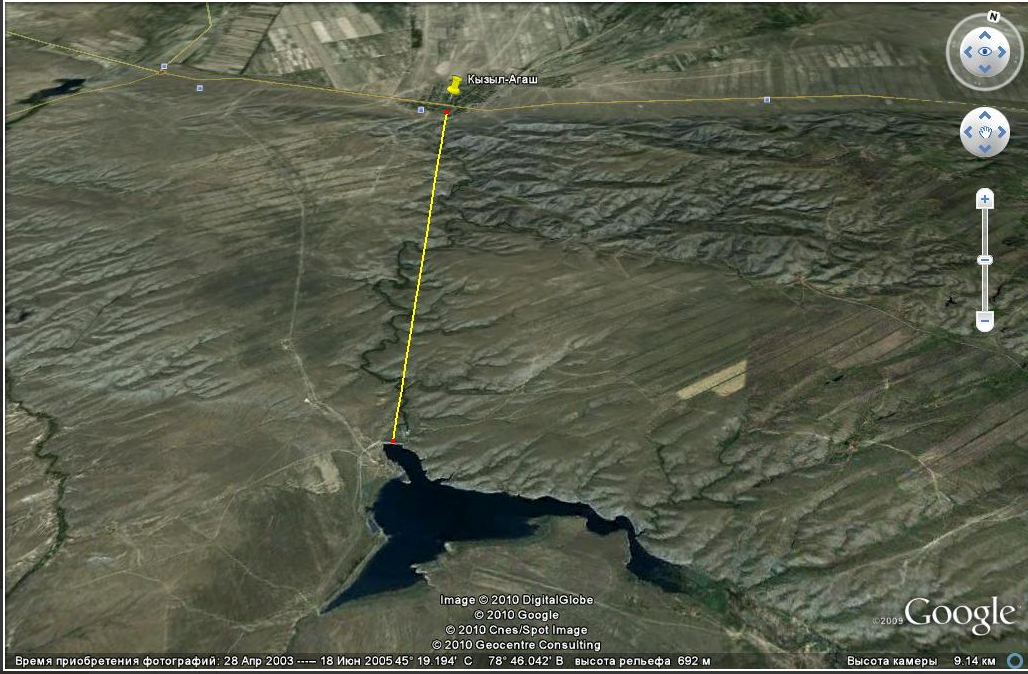
\includegraphics[width=0.8\textwidth]{media/ict/image3}
	\caption*{Рис. 2 - Расположение водоема и села Кызылагаш}
\end{figure}

\begin{multicols}{2}
В формуле (14) объем водохранилища (\(V_{2}\ \)) и высота до поверхности
воды \(h_{2}\) изменяются по времени; расстояние от створа плотины до
точки наблюдения (L) зависит от координат наблюдаемой точки.

\emph{{\bfseries Примечание.}} Полученная в работе (14) формула имеет
следующие границы применимости (связанные с методикой его обоснования):
объем водохранилища (\(V_{2}\)) -- от 3 млн.м\textsuperscript{3} и выше;
высота плотины (\(h_{0}\)) -- от 3 м и выше; расстояние от створа
плотины до створа наблюдения (L) -- от 3 м и выше. Указанные ограничения
не препятствуют практическим интересам.

{\bfseries Обсуждение и результаты.} Отсчет ведется каждые полчаса:

\[\mathrm{\Delta}T = 0.5 \text{ часа} = 30 \text{ минут}\]

Все дальнейшие расчеты моделируют события, произошедшие в селе Кызылагаш
Алматинской области 11 и 12 марта 2010 года. На рисунке 2 представлено
расположение села до указанной катастрофы. Дамба высотой 45 метров была
рассчитана на хранение 42 миллионов кубометров воды.

На основе разработанной автоматизированной системы была выполнена модель
событий, произошедших 11- 12 марта 2010 года в селе Кызылагаш. По данным
Алматинского департамента по чрезвычайным ситуациям, авария произошла
вследствие сильного дождя и повышения температуры воздуха. Эти условия
привели к движению льда и спровоцировали образование селевых потоков.

Ситуация, развившаяся в селе Кызылагаш, была смоделирована с
использованием формулы (14) и представлена на рисунке 3.
\end{multicols}

\begin{figure}[H]
	\centering
	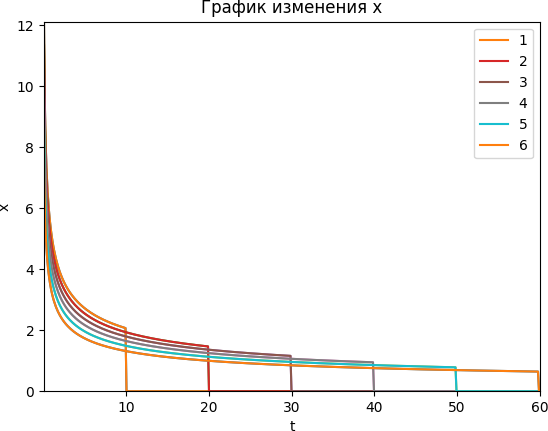
\includegraphics[width=0.6\textwidth]{media/ict/image4}
	\caption*{Рис. 3 - График максимальной волны прорыва в с.Кызылагаш}
\end{figure}

\begin{multicols}{2}
Согласно данным на рисунке, волна прорыва, достигшая села Кызылагаш в
течение одного часа, имела высоту 1.5 метра. За этот же промежуток
времени высота волны, выходящей из водоема, снизилась с 12 метров до 7
метров.

Таким образом, результаты численного моделирования подтверждаются
фактическими данными, зафиксированными в ходе события.

{\bfseries Выводы.} В рамках проведенного исследования достигнуты следующие
результаты:

1. разработана математическая модель для прогнозирования последствий
прорыва плотины. Создан алгоритм расчета максимального уровня волны
прорыва, учитывающий различные параметры гидротехнического сооружения.
Предложенный подход отличается высокой практической значимостью по
сравнению с существующими методами;

2. на языке Python создан программно-аппаратный комплекс (ПАК) для
мониторинга и прогнозирования последствий прорыва плотины;

3. на основе решения модельной задачи подтверждена эффективность
разработанного ПАК. В качестве практической основы была использована
ситуация, произошедшая в селе Кызылагаш Алматинской области Республики
Казахстан;

4. полученные результаты могут быть использованы для поддержки принятия
решений в органах управления водохозяйственной отрасли Казахстана.
Предложенные методика и технологии обеспечивают качественно новый
подход к задачам мониторинга водных ресурсов, выявлению явлений,
способствующих чрезвычайным ситуациям, и оценке их последствий.

\emph{{\bfseries Финансирование}. Работа выполнена за счет средств НИИ
математики и механики при КазНУ имени аль-Фараби и грантового
финансирования научных исследований на 2023--2025 годы по проекту
AP19678157.}
\end{multicols}

\begin{center}
{\bfseries Литература}
\end{center}

\begin{references}
1.Хамутова М.В., Кушников В.А. Математическая модель прогнозирования
последствий наводнений//Вестник Астрахан. гос. техн. ун-та. Серия
управление, вычисл. техн. информ.- 2016.- № 3. - С. 109-114.

2.Симагин И.М., Полуян Л.В. Моделирование зон возможных затоплений при
авариях на гидротехнических сооружениях. SAFETY2018. -- Екатеринбург,
2018. -- С. 14-21. \url{http://elar.urfu.ru/handle/10995/66329ю} Дата
обращения:17.12.2024

3.Стриганова М.Ю. Методы оценки и прогнозирование последствий при
разрушении гидротехнических сооружений // Вестник командно-инженерного
института МЧС Республики Белорусь.- 2012.- № 1(15). - С. 10-2.

4.Плеханов П.А. Гидрологические риски природного характера и их
предупреждение в Казахстане // Центрально-азиатский журнал исследований
воды. Специальный выпуск об опасностях, связанных с водой в Центральной
Азии. -- 2017. - № 3(1). - С. 19-25.

5.Молдабеков М.М., Еремир Д.И., Понятов Ю.А. Мониторинг уровня воды,
озер, рек морей и гидротехнических сооружений // Вестник КазНТУ.- 2013.
- №1. - С. 3-6.

6. Мазаков Т.Ж., Джомартова Ш.А., Мазакова А.Т., Шорманов Т.С., Алиаскар
М.С. Гибридная модель прогнозирования процесса селевого прорыва//Вестник
КазУТБ.-2024.- № 2(23). - С.1 20-126.
\href{https://doi.org/10.58805/kazutb.v.2.23-481}{DOI
10.58805/kazutb.v.2.23-481}

7.Мазаков Т.Ж., Джомартова Ш.А., Мазакова А.Т., Тойкенов Г.Ч., Алиаскар
М.С., Тойкенова У.Г. Идентификации математических моделей методом
квазилинераризации // Вестник КазУТБ. - 2024. - № 4(25).- C.16-23. DOI
10.58805/kazutb.v.4.25-650

8.Мазаков Т.Ж., Бургегулов А.Д., Джомартова Ш.А., Мазакова А.Т.,
Саметова А.А., Досаналиева А.Т. Построение маршрутов для эвакуации
сотрудников из здания при возникновении чрезвычайной ситуации // Вестник
КазУТБ. - 2024.- № 1(22).- C. 68-74

\href{https://doi.org/10.58805/kazutb.v.1.22-292}{DOI
10.58805/kazutb.v.1.22-292}
\end{references}

\begin{center}
{\bfseries References}
\end{center}

\begin{references}
1.Hamutova M.V., Kushnikov V.A. Matematicheskaja model'{}
prognozirovanija posledstvij navodnenij// Vestnik Astrahan. gos. tehn.
un-ta. Serija upravlenie, vychisl. tehn. inform.- 2016.- № 3. - S.
109-114. {[}in Russian{]}

2.Simagin I.M., Polujan L.V. Modelirovanie zon vozmozhnyh zatoplenij pri
avarijah na gidrotehnicheskih sooruzhenijah. SAFETY2018. --
Ekaterinburg, 2018. -- S. 14-21.
http://elar.urfu.ru/handle/10995/66329ju Data
obrashhenija:17.12.2024{[}in Russian{]}

3.Striganova M.Ju. Metody ocenki i prognozirovanie posledstvij pri
razrushenii gidrotehnicheskih \\sooruzhenij // Vestnik
komandno-inzhenernogo instituta MChS Respubliki
Belorus'.- 2012.- № 1(15). - S. 10-2. {[}in Russian{]}

4.Plehanov P.A. Gidrologicheskie riski prirodnogo haraktera i ih
preduprezhdenie v Kazahstane // Central' no-aziatskij
zhurnal issledovanij vody. Special' nyj vypusk ob
opasnostjah, svjazannyh s vodoj v Central' noj Azii. --
2017. - № 3(1). - S. 19-25. {[}in Russian{]}

5.Moldabekov M.M., Eremir D.I., Ponjatov Ju.A. Monitoring urovnja vody,
ozer, rek morej i \\gidrotehnicheskih sooruzhenij // Vestnik KazNTU.-
2013. - №1. - S. 3-6. {[}in Russian{]}

6. Mazakov T.Zh., Dzhomartova Sh.A., Mazakova A.T., Shormanov T.S.,
Aliaskar M.S. Gibridnaja model'{} prognozirovanija
processa selevogo proryva//Vestnik KazUTB.-2024.- № 2(23). - S.1 20-126.
DOI \\10.58805/kazutb.v.2.23-481{[}in Russian{]}

7.Mazakov T.Zh., Dzhomartova Sh.A., Mazakova A.T., Tojkenov G.Ch.,
Aliaskar M.S., Tojkenova U.G. Identifikacii matematicheskih modelej
metodom kvazilinerarizacii // Vestnik KazUTB. - 2024. - № 4(25).-
C.16-23. DOI 10.58805/kazutb.v.4.25-650{[}in Russian{]}

8.Mazakov T.Zh., Burgegulov A.D., Dzhomartova Sh.A., Mazakova A.T.,
Sametova A.A., \\Dosanalieva A.T. Postroenie marshrutov dlja jevakuacii
sotrudnikov iz zdanija pri vozniknovenii \\chrezvychajnoj situacii //
Vestnik KazUTB. - 2024.- № 1(22).- C. 68-74

DOI 10.58805/kazutb.v.1.22-292{[}in Russian{]}
\end{references}

\begin{authorinfo}
\emph{{\bfseries Сведения об авторах}}

Мазақова А.Т.- докторант КазНУ им.аль-Фараби, Алматы, Казахстан, e-mail:
\href{mailto:aigerym97@mail.ru}{\nolinkurl{aigerym97@mail.ru}}; ORCID:

https://orcid.org/0000-0003-3019-3352

Джомартова Ш.А. - доктор технических наук, доцент, КазНУ им. аль-Фараби,
Алматы, Казахстан, e-mail:\\
\href{mailto:jomartova@mail.ru}{\nolinkurl{jomartova@mail.ru}}; ORCID:
https://orcid.org/0000-0002-5882-5588

Мазақова Б.М. -- cт.преп. \emph{Казахский агротехнический}
исследовательский \emph{университет} имени С. Сейфуллина, Астана,
Казахстан, e-mail:
\href{mailto:bayan7080@mail.ru}{\nolinkurl{bayan7080@mail.ru}};
ORCID: https://orcid.org/0000-0003-4904-3557

Әлиасқар М.С. - старший преподаватель МИТУ, Алматы, Казахстан, e-mail:
\href{mailto:m.alyasqar@gmail.ru}{\nolinkurl{m.alyasqar@gmail.ru}};
ORCID:

\href{https://orcid.org/0000-0002-3013-6617}{https://orcid.org/0000-0002-3013-6617}

Мергенгали Е.К. -- докторант КазНУ имени аль-Фараби, Алматы, Казахстан,
e-mail:
\href{https://e.mail.ru/compose/?mailto=mailto\%3aestony.9999@gmail.com}{estony.9999@gmail.com};
ORCID: \\https://orcid.org/0000-0002-9755-6472

Мазаков Т.Ж. - доктор физико-математических наук, профессор, КазНУ им.
аль-Фараби, Алматы, Казахстан, e-mail:
\href{mailto:tmazakov@mail.ru}{\nolinkurl{tmazakov@mail.ru}}; ORCID:
https://orcid.org/ 0000-0001-9345-5167

Досаналиева А.Т. - сеньор-лектор кафедры «Компьютерная инженерия»
Алматинского технологического Университета, Алматы, Казахстан, e-mail:
\href{mailto:Dosanalieva1985@gmail.com}{\nolinkurl{Dosanalieva1985@gmail.com}};
ORCID: \url{https://orcid.org/0009-0000-2958-1935}

Майлыбаева А.Д. -- к.ф.-м.н., доцент кафедры «Информатика» Атырауского
универститета имени Х. Досмухамедова, Атырау, Казахстан, e-mail:
\href{mailto:a.maylibayeva@asu.edu.kz}{\nolinkurl{a.maylibayeva@asu.edu.kz}};
ORCID: 0000-0003-0598-4806

\emph{{\bfseries Information about the author}}

Mazakova A.T.- Doctoral student of Al-Farabi Kazakh National University,
Almaty, Kazakhstan, e-mail:
\href{mailto:aigerym97@mail.ru}{\nolinkurl{aigerym97@mail.ru}};

Jomartova Sh.A. - Doctor of Technical Sciences, Associate Professor,
Al-Farabi KazNU, Almaty, Kazakhstan, e-mail:\\
\href{mailto:jomartova@mail.ru}{\nolinkurl{jomartova@mail.ru}};

Mazakova B.M. - Senior Lecturer, Kazakh Agrotechnical Research
University named after S. Seifullin, Astana, Kazakhstan, e-mail:
\href{mailto:bayan7080@mail.ru}{\nolinkurl{bayan7080@mail.ru}};

Aliaskar M.S. - Senior Lecturer, MITU, Almaty, Kazakhstan, e-mail:
\href{mailto:m.alyasqar@gmail.ru}{\nolinkurl{m.alyasqar@gmail.ru}};

Mergengali E.K. - Doctoral student of Al-Farabi Kazakh National
University, Almaty, Kazakhstan, e-mail:\\
\href{mailto:estony.9999@gmail.com}{\nolinkurl{estony.9999@gmail.com}};

Mazakov T.Zh. - Doctor of Physical and Mathematical Sciences, Professor,
Al-Farabi KazNU, Almaty, Kazakhstan, e-mail:
\href{mailto:tmazakov@mail.ru}{\nolinkurl{tmazakov@mail.ru}};

Dosanalieva A.T. - Senor Lecturer, Computer Engineering Department,
Almaty Technological University, Almaty, Kazakhstan, e-mail:
\href{mailto:Dosanalieva1985@gmail.com}{\nolinkurl{Dosanalieva1985@gmail.com}}

Mailybayeva A.D. - PhD, Associate Professor, Department of Computer
Science, Atyrau University named after Kh. \\Dosmukhambetov, Atyrau,
Kazakhstan, e-mail:
\href{mailto:a.maylibayeva@asu.edu.kz}{\nolinkurl{a.maylibayeva@asu.edu.kz}};
ORCID: https://orcid.org/0000-0003-0598-4806
\end{authorinfo}
